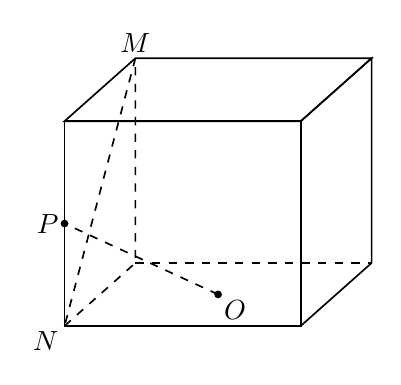
\begin{tikzpicture}[x=1cm,y=1cm,font=\normalsize]
% Cube, MN left-face diagonal (dashed), OP interior (dashed)
\coordinate (FBL) at (0,0);
\coordinate (FBR) at (3,0);
\coordinate (FTR) at (3,2.6);
\coordinate (FTL) at (0,2.6);
\coordinate (BBL) at (0.9,0.8);
\coordinate (BBR) at (3.9,0.8);
\coordinate (BTR) at (3.9,3.4);
\coordinate (BTL) at (0.9,3.4);
\coordinate (M) at (0.9,3.4);
\coordinate (N) at (0,0);
\coordinate (O) at (1.95,0.4);
\coordinate (P) at (0,1.3);
\draw[line width=.6pt] (FBL)--(FBR)--(FTR)--(FTL)--cycle;
\draw[line width=.6pt] (FTL)--(FTR)--(BTR)--(BTL)--cycle;
\draw[line width=.6pt] (FTR)--(BTR)--(BBR)--(FBR);
\draw[line width=.6pt,dashed] (BBL)--(BBR);
\draw[line width=.6pt,dashed] (FBL)--(BBL)--(BTL);
\draw[line width=.6pt,dashed] (M)--(N);
\draw[line width=.6pt,dashed] (O)--(P);
\fill (O) circle (1.4pt);
\fill (P) circle (1.4pt);
\node[inner sep=2pt,above] at (M) {$M$};
\node[inner sep=2pt,below left] at (N) {$N$};
\node[inner sep=2pt,below right] at (O) {$O$};
\node[inner sep=2pt,left] at (P) {$P$};
\end{tikzpicture}
